\documentclass[./main.tex]{subfiles}

\begin{document}
\chapter{IMPLEMENTATION}
\addtocontents{lof}{\protect\addvspace{-10pt}}
\addtocontents{lot}{\protect\addvspace{-10pt}}
\noindent
Implementation is the stage of the project when the theoretical design is turned out into a working system. Thus it can be considered to be the most critical stage in achieving a successful new system and in giving the user, confidence that the new system will work and be effective. The implementation stage involves careful planning, investigation of the existing system and it’s constraints on implementation, designing of methods to achieve changeover and evaluation of changeover methods.
\section{Tools and Technologies}
\subsection {Languages and Frameworks}
\begin{enumerate}[label=\ensuremath{\diamond}]
  \item \textbf{Python}: Python is an interpreted, high-level and general-purpose programming language. Python's design philosophy emphasizes code readability with its notable use of significant indentation. Its language constructs and object-oriented approach aim to help programmers write clear, logical code for small and large-scale projects. Python is dynamically typed and garbage-collected. It supports multiple programming paradigms, including structured (particularly, procedural), object-oriented, and functional programming. Python is often described as a "batteries included" language due to its comprehensive standard library. 
  \item \textbf {Google Collab}: Google Colab is a free cloud service and now it supports free GPU! You can; improve your Python programming language coding skills. develop deep learning applications using popular libraries such as Keras, TensorFlow, PyTorch, and OpenCV.
  \item \textbf{Scikit Learn}: Scikit-learn is a free software machine learning library for the Python programming language. It features various classification, regression and clustering algorithms including support vector machines, random forests, gradient boosting, k-means and DBSCAN, and is designed to interoperate with the Python numerical and scientific libraries NumPy and SciPy.
  \item \textbf{TensorFlow}: TensorFlow is a free and open-source software library for machine learning. It can be used across a range of tasks but has a particular focus on training and inference of deep neural networks. Tensorflow is a symbolic math library based on dataflow and differentiable programming.
  \item \textbf{Django}: Django is a Python-based free and open-source web framework that follows the model-template-views architectural pattern. It is maintained by the Django Software Foundation. Django's primary goal is to ease the creation of complex, database-driven websites. \cite{python}
\end{enumerate}
\subsection {CASE Tools}
\begin{enumerate}[label=\ensuremath{\diamond}]
  \item \textbf{Draw.io}: Draw.io is a free online diagram software for making flowcharts, process diagrams, org charts, UML, ER and network diagrams.
  \item \textbf{Vs-Code}: Visual Studio Code is a free source-code editor made by Microsoft for Windows, Linux and macOS. Features include support for debugging, syntax highlighting, intelligent code completion, snippets, code refactoring, and embedded Git.
  \item \textbf{Git}: Git is a free and open source distributed version control system designed to handle everything from small to very large projects with speed and efficiency.
  \item \textbf{Trello}: Trello is a web-based Kanban-style list-making application which is a subsidiary of Atlassian. 
  \end {enumerate}
\section{Working Of LSTM Algorithm}
The Long Short-Term Memory (LSTM) network is a type of recurrent neural network (RNN) designed to address the vanishing gradient problem that occurs in traditional RNNs. Here is a high-level mathematical derivation of the LSTM update equations.
\noindent
Let's consider an LSTM cell at time step \(t\). The LSTM cell maintains a cell state (\(c_t\)), hidden state (\(h_t\)), input gate (\(i_t\)), forget gate (\(f_t\)), output gate (\(o_t\)), and memory cell content (\(g_t\)). The update equations for these components are given by:

1. \textbf{Input Gate (\(i_t\)):}
   \[ i_t = \sigma(W_{ii}x_t + b_{ii} + W_{hi}h_{t-1} + b_{hi}) \]

2. \textbf{Forget Gate (\(f_t\)):}
   \[ f_t = \sigma(W_{if}x_t + b_{if} + W_{hf}h_{t-1} + b_{hf}) \]

3. \textbf{Output Gate (\(o_t\)):}
   \[ o_t = \sigma(W_{io}x_t + b_{io} + W_{ho}h_{t-1} + b_{ho}) \]

4. \textbf{Cell State Update (\(g_t\)):}
   \[ g_t = \tanh(W_{ig}x_t + b_{ig} + W_{hg}h_{t-1} + b_{hg}) \]

5. \textbf{Cell State (\(c_t\)) Update:}
   \[ c_t = f_tc_{t-1} + i_tg_t \]

6. \textbf{Hidden State (\(h_t\)) Update:}
   \[ h_t = o_t\tanh(c_t) \]

In these equations:

\begin{itemize}
  \item \(x_t\) is the input at time step \(t\).
  \item \(W_{ii}, W_{hi}, b_{ii}, b_{hi}\) are weight matrices and bias terms for the input gate.
  \item \(W_{if}, W_{hf}, b_{if}, b_{hf}\) are weight matrices and bias terms for the forget gate.
  \item \(W_{io}, W_{ho}, b_{io}, b_{ho}\) are weight matrices and bias terms for the output gate.
  \item \(W_{ig}, W_{hg}, b_{ig}, b_{hg}\) are weight matrices and bias terms for the cell state update.
  \item \(\sigma\) represents the sigmoid activation function, and \(\tanh\) represents the hyperbolic tangent activation function.
\end{itemize}
\noindent
These equations describe how information is updated and propagated through the LSTM cell at each time step. The input gate controls how much of the new information should be added to the cell state, the forget gate controls how much of the previous cell state should be retained, and the output gate controls how much of the cell state should be exposed to the next layer.
\noindent
This architecture allows LSTMs to capture and remember long-term dependencies in sequential data, making them suitable for tasks such as natural language processing, time series prediction, and more. \cite{olah2015understanding}

\subsection{High Level Overview Of LSTM algorithm}
\begin{enumerate}
    \item \textbf{Import Libraries:}
    \begin{lstlisting}[frame=single, language=python,basicstyle=\small\ttfamily,breaklines=true,showspaces=false,columns=fullflexible, literate={\ }{{\ }}1]
        import numpy as np
        import tensorflow as tf
        from tensorflow.keras.models import Sequential
        from tensorflow.keras.layers import LSTM, Dense
        \end{lstlisting}

    \item \textbf{Prepare Sequential Data:}
        \begin{lstlisting}[frame=single, language=python]
        # Example: Generate sequential data
        sequence_length = 10
        X_train = np.random.rand(100, sequence_length, 1)
        y_train = np.random.randint(0, 2, size=(100,))
        \end{lstlisting}

    \item \textbf{Build LSTM Model:}
        \begin{lstlisting}[frame=single, language=python]
        model = Sequential()
        model.add(LSTM(units=50, 
            input_shape=(sequence_length, 1)))
        model.add(Dense(units=1, activation='sigmoid'))
        \end{lstlisting}

    \item \textbf{Compile the Model:}
        \begin{lstlisting}[frame=single, language=python]
        model.compile(optimizer='adam',
        loss='binary_crossentropy', metrics=['accuracy'])
        \end{lstlisting}

    \item \textbf{Train the Model:}
        \begin{lstlisting}[frame=single, language=python]
        model.fit(X_train,y_train,epochs=10,batch_size=32)
        \end{lstlisting}

    \item \textbf{Make Predictions:}
        \begin{lstlisting}[frame=single, language=python]
        X_test = np.random.rand(10, sequence_length, 1)
        predictions = model.predict(X_test)
        \end{lstlisting}

    \item \textbf{Evaluate the Model:}
        \begin{lstlisting}[frame=single, language=python]
        # Example: Generate test data
        X_test = np.random.rand(20, sequence_length, 1)
        y_test = np.random.randint(0, 2, size=(20,))

        # Evaluate the model
        loss, accuracy = model.evaluate(X_test, y_test)
        print(f"TestLoss: {loss},TestAccuracy: {accuracy}")
        \end{lstlisting}
\end{enumerate}


% \section{Expected Outcome}
% The expected outcome of this project is to develop a user-friendly Stock Forecasting system that equips investors with accurate stock predictions and risk management tools. Through extensive research and the integration of the latest trends in finance and stock prediction, this system aims to provide users with the means to make informed investment decisions. Ultimately, it will enable users to potentially enhance their profitability and reduce financial risks while navigating the dynamic world of stock trading.
\section{Testing}
Testing is the process of evaluating a system or its component(s) with the intent to find whether it satisfies the specified requirements or not. Testing is executing a system in order to identify any gaps, errors, or missing requirements in contrary to the actual requirements. 
\begin{center}
\begin{table}[H]
  \caption{Algorithm Testing}
  \begin{tabular}{|c|c|c|c|c|c|}
    \hline
    \textbf{sn} & \textbf{Stock Symbol} &\textbf{LTP} & \textbf{Actual Opening Price} & \textbf{Predicted Opening Price} & \textbf{Difference}  \\
    \hline
    1 & NABIL & 491.20 & 497 & 502 & +5\\
    2 & ACLBSL & 607.00 & 610 & 606 & -4  \\
    3 & ADBL & 245.10 & 245 & 238 & -7\\
    \hline
  \end{tabular}
\end{table}
\end{center}
\subsection*{Accuracy of the model}
The model is trained with NEPSE stock datas and tested with the same data. The 180 days data is divided into training and testing parts in the ratio of 80:20. The model is trained with 80\% of the data and tested with 20\% of the data.
After training, the LSTM algorithm achieved an accuracy of 72\% on the testing data, using a threshold of 0.85 for classifying stock movements as "up" or "down". This accuracy indicates the model's ability to make accurate predictions on unseen data. Additionally, performance metrics such as precision, recall, and F1-score can provide further insights into the model's performance and its ability to correctly classify stock movements.
\newline \noindent \textbf{Precision:} Precision measures the proportion of true positive predictions among all positive predictions made by the model. It is calculated as the ratio of true positives to the sum of true positives and false positives.

\[ Precision = \frac{TP}{TP + FP} \]
\noindent \textbf{False Positive Rate (FPR):} FPR measures the proportion of false positive predictions among all actual negative instances in the dataset. It is calculated as the ratio of false positives to the sum of false positives and true negatives.

\[ FPR = \frac{FP}{TN + FP} \]

\noindent \textbf{Balanced Accuracy:} Balanced accuracy calculates the average of sensitivity and specificity and is suitable for imbalanced datasets.

\[ Balanced \ Accuracy = \frac{1}{2} \cdot (Sensitivity + Specificity) \]
\newline \noindent \textbf{F1 Score}: The F1 score is the harmonic mean of precision and recall, providing a single metric that balances both measures. It is calculated as
\[ F1 \ Score = 2 \times \frac{Precision \times Recall}{Precision + Recall} \]
\noindent
\textbf{Precision:} 0.722 \\
\textbf{F1 Score:} 0.8387 \\
\textbf{Accuracy:} 0.722 \\
\textbf{Balanced Accuracy:} 0.5 \\



\begin{figure}[H]
    \centering
    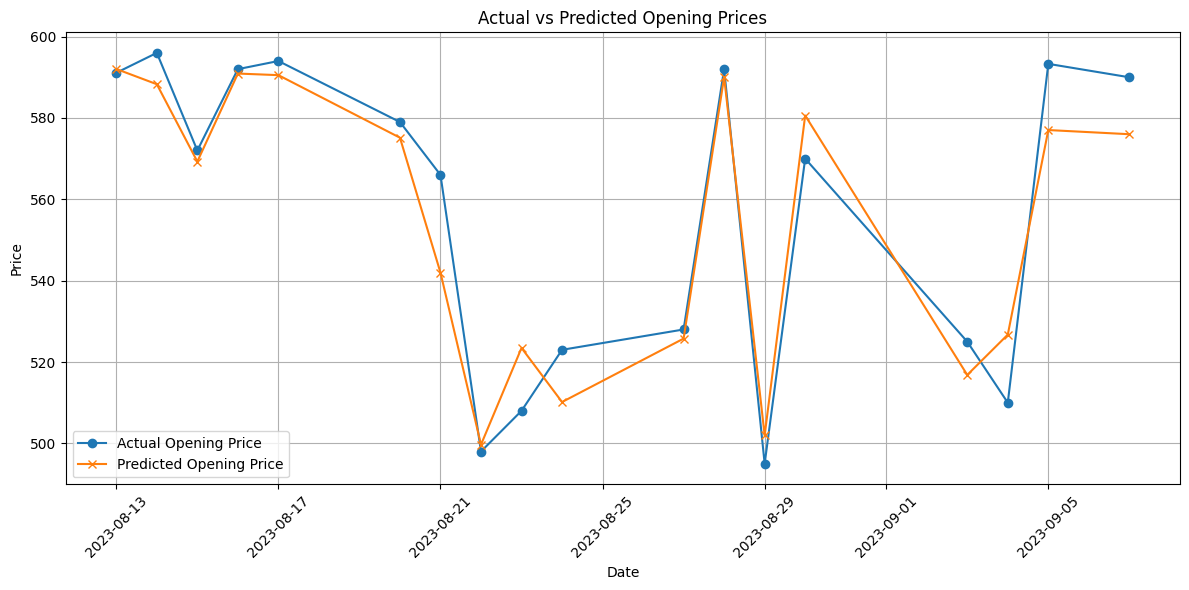
\includegraphics[width=1\linewidth]{images/Algorithmtesting.png}
    \caption{Algorithm Testing}
    \label{fig:5.1}
\end{figure}
\section{User Acceptance Testing}
\begin{center}
\begin{table}[H]
  \caption{User Acceptance Testing}
  \begin{tabular}{|c|c|c|c|c|}
    \hline
    \textbf{sn} & \textbf{Can Train} &\textbf{Expected Outcome} &\textbf{Can Visualize} & \textbf{Test Result}   \\
    \hline
    1 & Yes & Yes &Yes & Pass\\
    2 & Yes & Yes &Yes & Pass\\
    3 & Yes & Yes &Yes & Pass \\
    \hline
  \end{tabular}
\end{table}
\end{center}
\end{document}